\subsection{Normalized Mutual Information evolution for a big dataset}
	
	This dataset is made from 75000 combinations of 9 zernike modes their RMSE ranging from:
	\begin{itemize}
		\item Modes 2,3 between [-0.8, 0.8]
		\item Modes 4,5,6 between [-0.6, 0.6]
		\item Modes 7,8,9,10 between [-0.4, 0.4]
	\end{itemize}
	
	\subsubsection{NMI evolution over number of clusters for 9 zernike mode related datasets}
		\begin{figure*}[ht!]
			\centering
			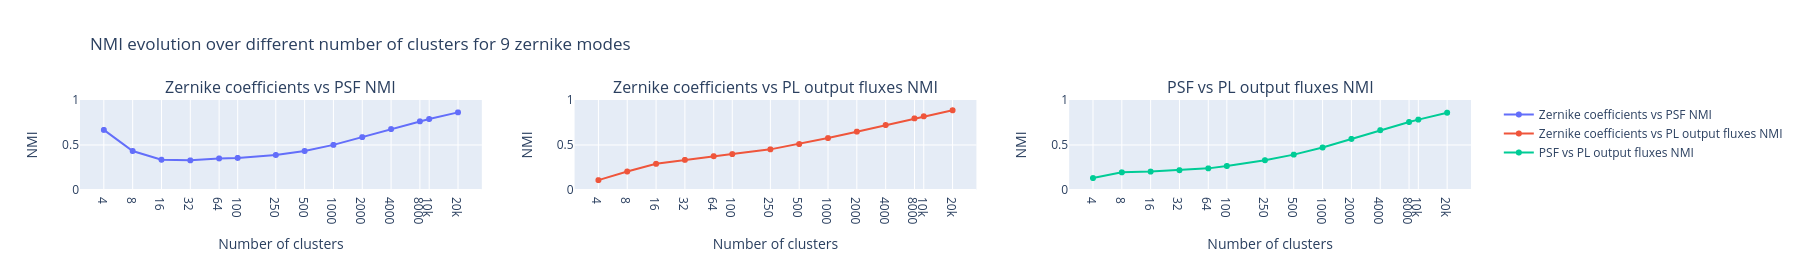
\includegraphics[width=0.9\textwidth]{nmia-nmievolutionoverbig9.png}
		\end{figure*}
		
\begin{table}[h!]
\centering
\begin{tabular}{|c|c|c|c|}
\hline
\textbf{Clusters} & \textbf{Z vs PSF} & \textbf{Z vs PL} & \textbf{PSF vs PL} \\
\hline
4 & 0.667 & 0.109 & 0.133 \\
8 & 0.433 & 0.205 & 0.196 \\
16 & 0.336 & 0.291 & 0.205 \\
32 & 0.329 & 0.334 & 0.220 \\
64 & 0.351 & 0.375 & 0.240 \\
100 & 0.356 & 0.399 & 0.267 \\
250 & 0.389 & 0.452 & 0.331 \\
500 & 0.433 & 0.510 & 0.393 \\
1000 & 0.501 & 0.577 & 0.472 \\
2000 & 0.588 & 0.648 & 0.567 \\
4000 & 0.677 & 0.722 & 0.664 \\
8000 & 0.763 & 0.796 & 0.755 \\
10000 & 0.789 & 0.819 & 0.782 \\
20000 & 0.863 & 0.886 & 0.859 \\
\hline
\end{tabular}
\caption{NMI Analysis for Different Numbers of Clusters}
\end{table}